\section{Validation of PPM implementation}
% \begin{frame}
% \frametitle{Inverse dielectric}
% \begin{figure}
%     \centering
%     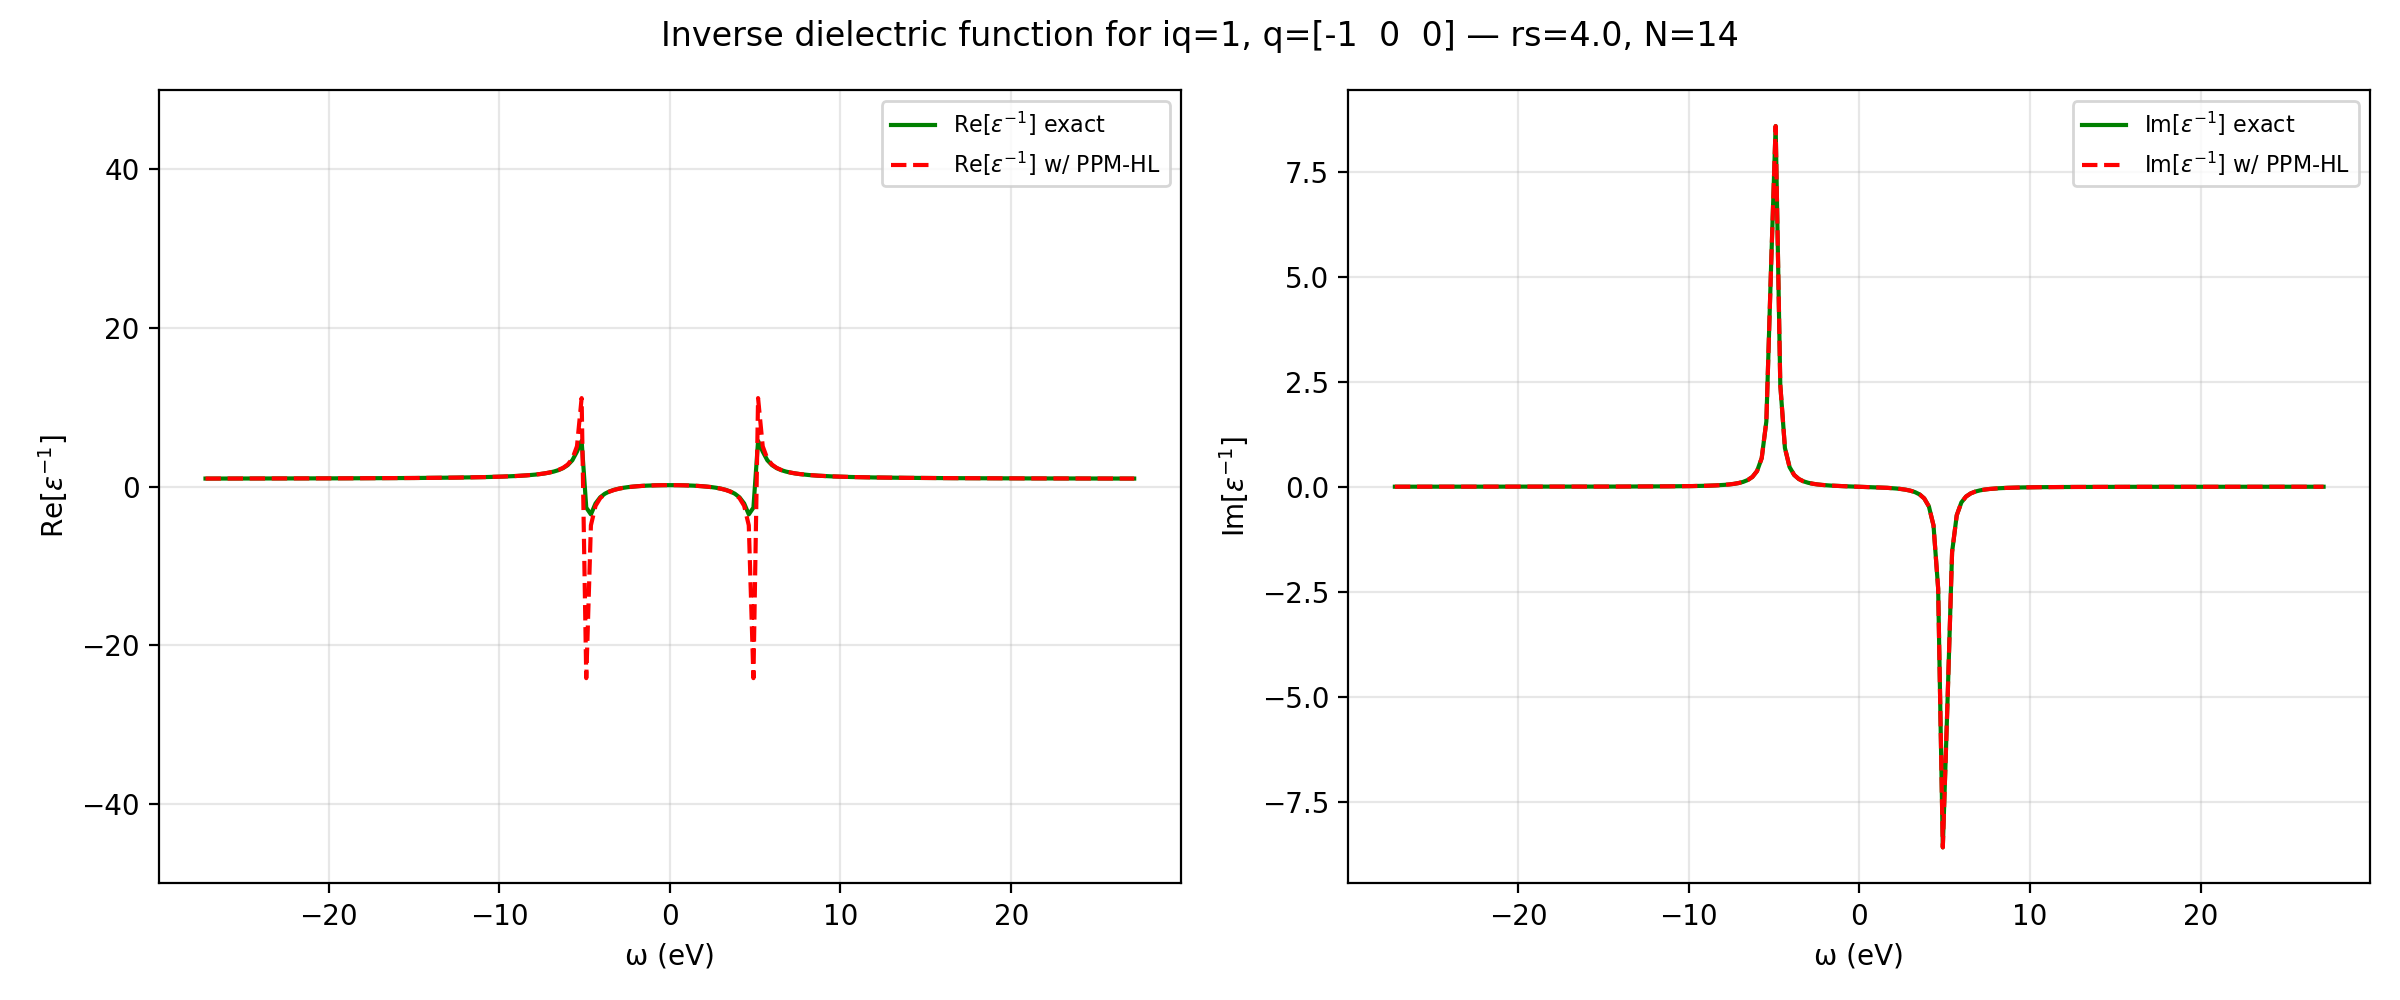
\includegraphics[width=\textwidth]{figs/5-22/inverse_dielectric_LDA_q1_rs4.png}
% \end{figure}
% \end{frame}
\begin{frame}
    \frametitle{Equivalence between dynamical COHSEX and GW}
We can partition $ \Sigma^{\mathrm{GW}}=\Sigma_{\mathrm{SEX}}+\Sigma_{\mathrm{COH}}$ with \pause
\begin{align}
\Sigma_{G G}^{\mathrm{SEX}}(\omega )
&= -\frac{1}{\Omega} \sum_{G_n}^{\mathrm{occ}} \left(\underbrace{1}_{\Sigma^x}+\frac{\Omega_{G-G_n, G-G_n}^2}{\left(\omega-\varepsilon_{G_n}\right)^2-\tilde{\omega}_{G-G_n, G-G_n}^2}\right) v\left(G-G_n\right)
\end{align}
\pause and
\begin{align}
\Sigma_{G G}^{\mathrm{COH}}(\omega )
&= \frac{1}{2\Omega} \sum_{G_n}  \frac{\Omega_{G-G_n, G-G_n}^2}{\tilde{\omega}_{G-G_n, G-G_n}\left[\omega-\varepsilon_{G_n}-\tilde{\omega}_{G-G_n, G-G_n}\right]} v\left(G-G_n\right)
\end{align}
\end{frame}
\begin{frame}
\frametitle{Self energy}
\begin{figure}
    \centering
    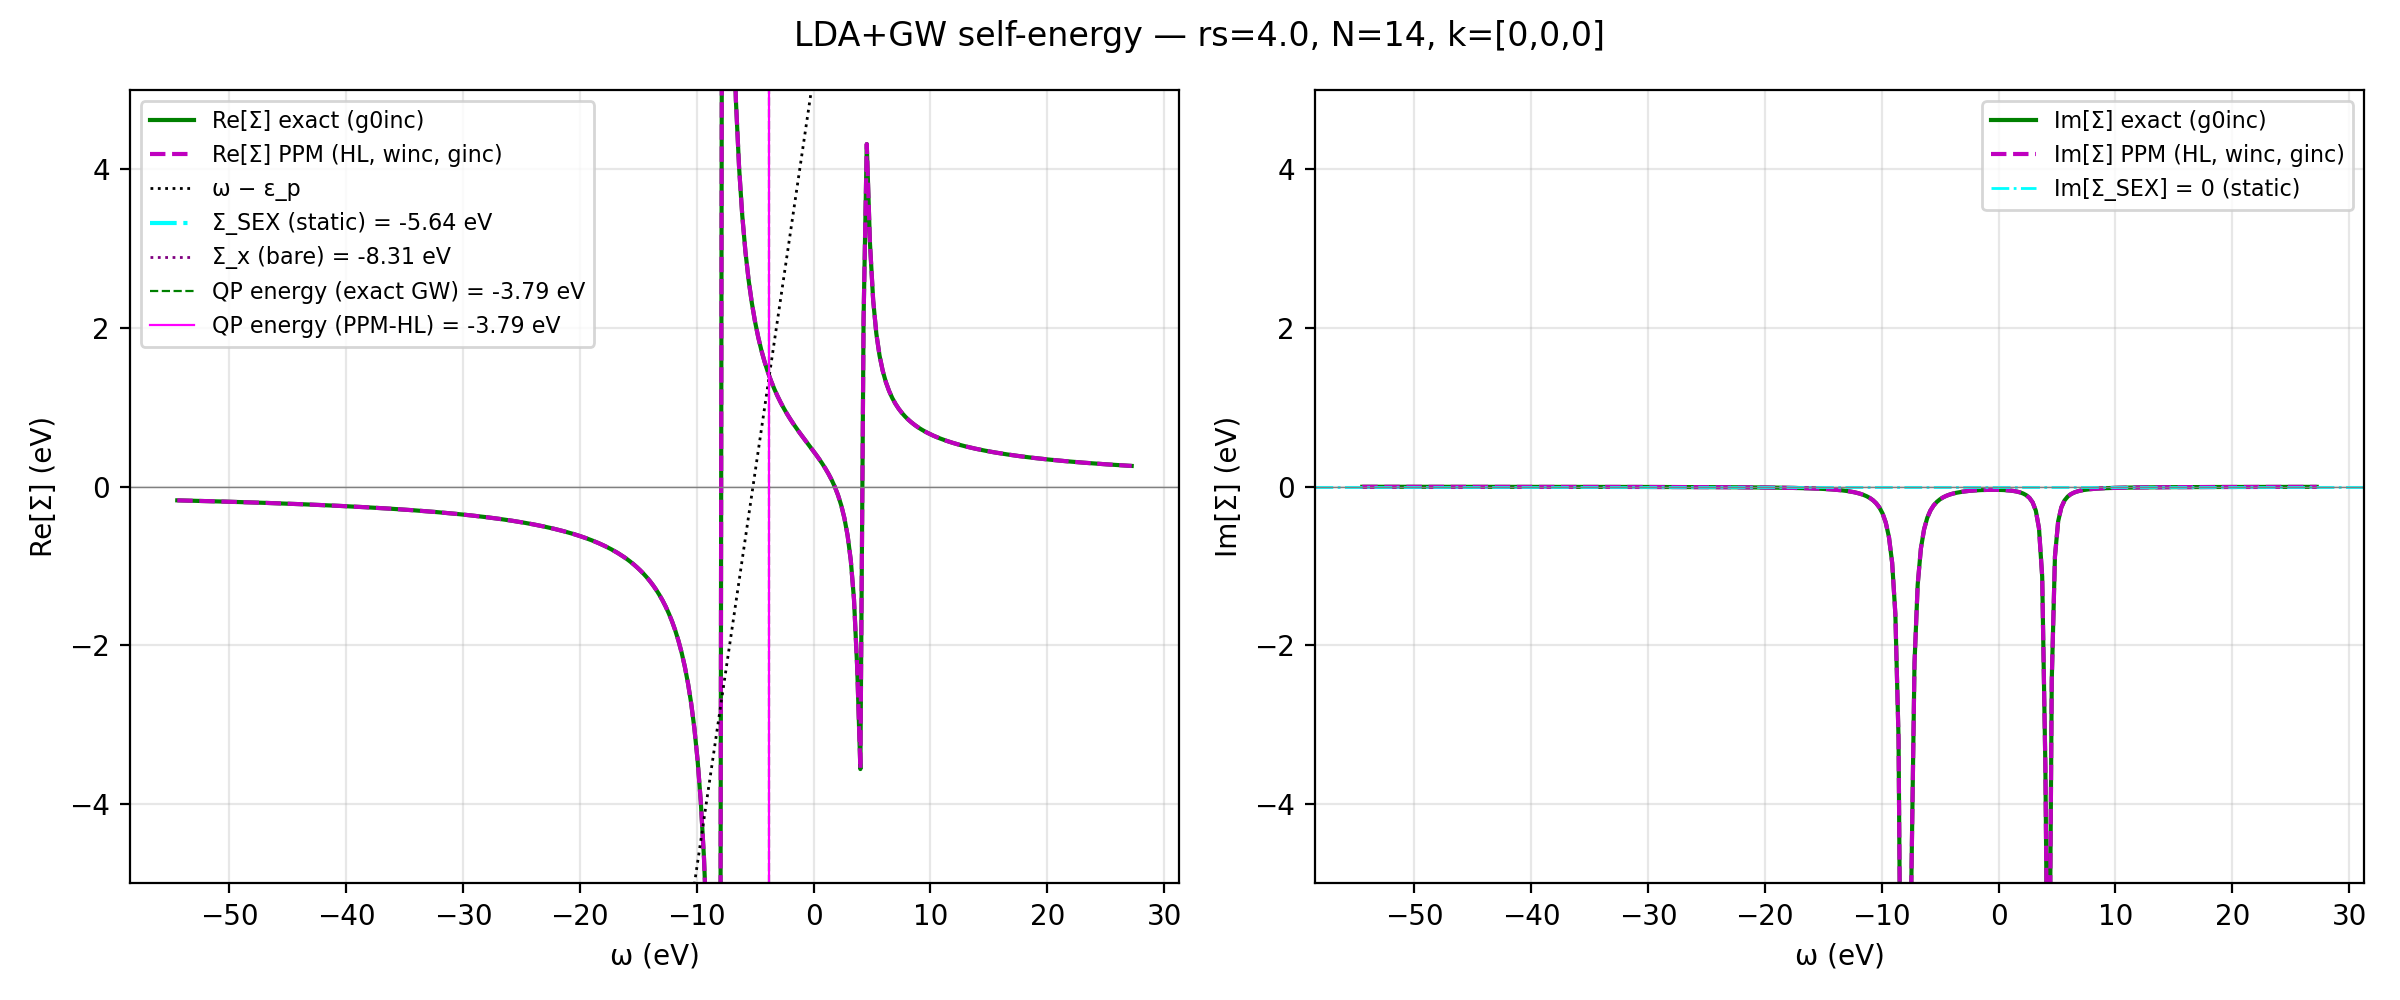
\includegraphics[width=\textwidth]{figs/5-22/selfenergy_LDA_rs4.0_pidx0.png}
\end{figure}
PPMs use the dynamical COHEX self-energy expression
\end{frame}
\begin{frame}   
\frametitle{What I fixed}
We know
\begin{align}
\Omega_{G G^{\prime}}^2(q)=\omega_p^2 \frac{(q+G) \cdot\left(q+G^{\prime}\right)}{|q+G|^2} \frac{n\left(G-G^{\prime}\right)}{n(0)}\overset{UEG}{=}\omega _p^2 \overset{TDL}{=} 4\pi n 
\end{align}
\pause
But in the finite sized system, we actually have 
\begin{equation}
    \Omega_{\mathbf{q}}^2
    =
    \frac{4v_{\mathbf{q}}}{V}
    \sum_{(i,a)\in\mathcal{T}_{\mathbf{q}}}
    \left(\varepsilon_a-\varepsilon_i\right),
\end{equation}
\pause
This follows from a need to satisfy the f-sum rule as 
\begin{equation}
\int_{-\infty}^{\infty} \omega \operatorname{Im} \varepsilon^{-1}(\mathbf{q}, \omega) d\omega = -\pi \Omega^2(\mathbf{q}).
\end{equation}
\end{frame}
\section{Time-ordering as the remaining discrepancy}
\begin{frame}
\frametitle{Theory}
We have
% $\begin{aligned} A_{p q}(\omega) & =\frac{\mathrm{i}}{2 \pi}\left[G_{p q}^{>}(\omega)-G_{p q}^{<}(\omega)\right] \\ & =\frac{1}{\pi}\left|\operatorname{Im} G_{p q}^{\mathrm{T}}(\omega)\right|=-\frac{1}{\pi} \operatorname{Im} G_{p q}^{\mathrm{R}}(\omega)\end{aligned}$
\begin{equation}
    A_{p q}(\omega) =\frac{1}{\pi}\left|\operatorname{Im} G_{p q}^{\mathrm{T}}(\omega)\right|=-\frac{1}{\pi} \operatorname{Im} G_{p q}^{\mathrm{R}}(\omega)
\end{equation}\pause
with
\begin{equation}
    G^{\text{TO}}_k(t) = i\Theta(-t) e^{-i \varepsilon^0_k t} \exp \left[-i \Sigma_k^{\mathrm{x}} t+C_k^h(t)\right]
\end{equation}\pause
and
\begin{equation}
    C_k^h(t)=\frac{1}{\pi} \int_{-\infty}^0 d \omega \frac{\left|\operatorname{Im} \Sigma_k^R\left(E_k^{G W}+\omega\right)\right|}{\omega^2}\left(e^{-i \omega t}+i \omega t-1\right).
\end{equation}
\end{frame}
\begin{frame}
\frametitle{Results}
\begin{figure}
    \centering
    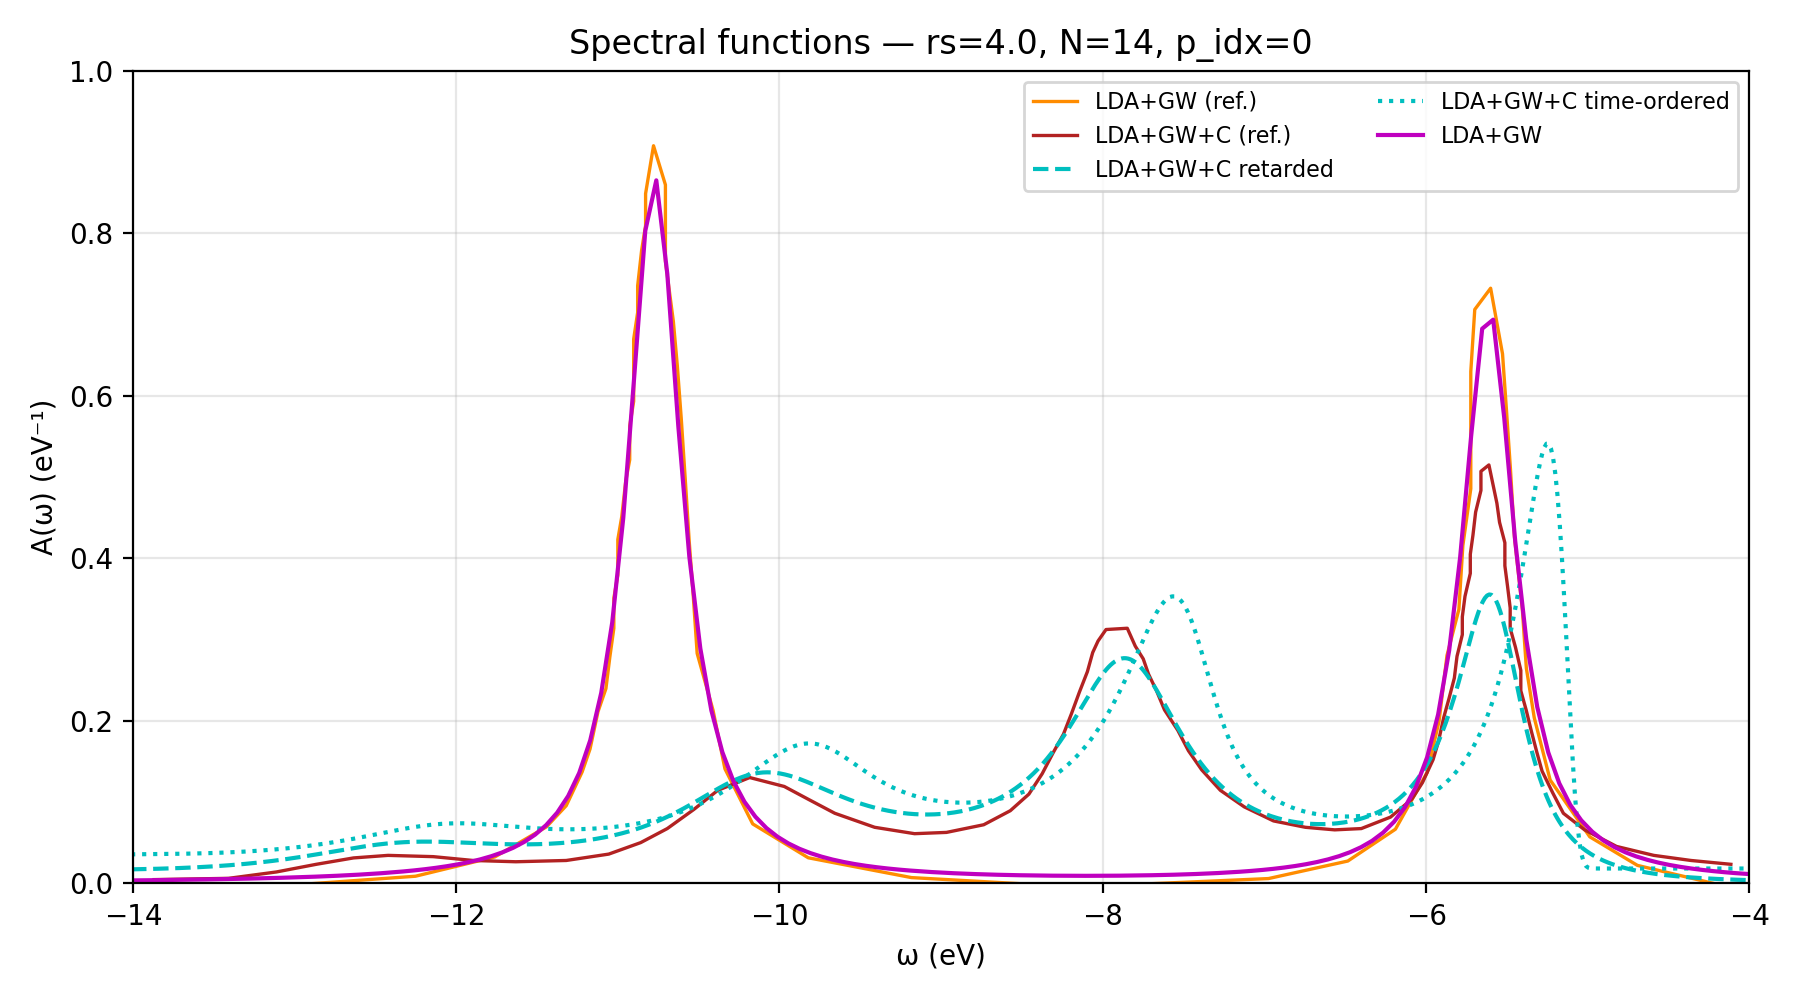
\includegraphics[width=\textwidth]{figs/5-22/comparison_LDA_0.png}
\end{figure}
\end{frame}
\section{Discuss choice of committee}
\begin{frame}
\frametitle{Discuss choice of committee}
\end{frame}
